
\chapter{Introduzione}
L'obiettivo del progetto realizzato è quello di integrare la libreria OROCOS KDL (\url{https://www.orocos.org/kdl.html}) nel component framework \textit{STAR} per definire un'applicazione che consente di inviare al robot comandi di posizione della pinza montata all'estremità del robot manipolatore P-Rob 3 (\Fig\ref{fig:prob3}) rispetto al sistema di riferimento cartesiano alla base del robot.
\begin{figure}[b!]
	\centering
	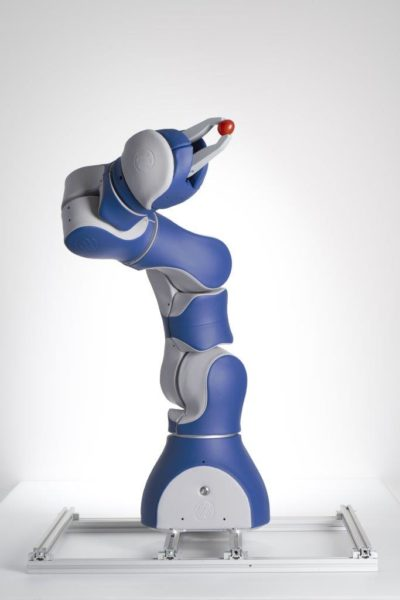
\includegraphics[width=0.4\linewidth]{./ImageFiles/P-Rob 3.jpg}
	\caption{Robot manipolatore P-Rob 3.}
	\label{fig:prob3}
\end{figure}
In particolare, si sono sviluppate le seguenti funzionalità:
\begin{itemize}
	\item calcolo della posizione della pinza rispetto al sistema di riferimento alla base del robot a partire dal valore degli angoli dei giunti (cinematica diretta);
	\item calcolo del valore dei giunti a partire dalla posizione della pinza rispetto al sistema di riferimento alla base del robot (cinematica inversa);
	\item calcolo di un percorso lineare a partire da una posizione iniziale e una finale della pinza.
\end{itemize}

\chapter{Libreria OROCOS KDL}
\section{Installazione}
Per effettuare i calcoli cinematici si è scelto di utilizzare la libreria OROCOS KDL, che implementa le funzionalità base come il calcolo della cinematica diretta e inversa per un robot. Seguendo la guida di installazione disponibile nella documentazione (\url{https://www.orocos.org/wiki/Installation_Manual.html}), la libreria è stata installata nel framework \textit{STAR} al seguente percorso: STAR/AutonomousRobot/Libraries/others/orocos\_kinematics\_dynamics. Inoltre, per semplificare alcune operazioni di inizializzazione della libreria KDL, è stato installata la libreria \textit{kdl parser} nella cartella STAR/AutonomousRobot/Libraries/others/kdl\_parser, seguendo le istruzioni di installazione reperibili al seguente link \url{STAR/AutonomousRobot/Libraries/others/orocos\_kinematics\_dynamics}. Infine, è stato modificato il file \textit{ev-star.sh} inserendo le informazioni per includere i file e recuperare i binari delle librerie installate quando vengono compilati componenti e plugin.

\section{Definizione del modello del robot}
La libreria KDL ha bisogno di conoscere la struttura cinematica del robot. La catena cinematica del robot è stata definita in un file .urdf (\url{http://wiki.ros.org/urdf}), nel quale sono descritti in modo standard tutti i parametri, quali ad esempio il numero, la tipologia e i limiti dei giunti e la lunghezza dei link. Per definire questo file, si è partiti dal modello fornito sulla pagina github del produttore (\url{https://github.com/fp-robotics/fp_descriptions}), generando il file urdf seguendo la procedura indicata. Successivamente, il file è stato modificato per estrapolare le informazioni rilevanti per il progetto e, eseguendo delle prove con l'interfaccia web fornita dal produttore del robot, sono stati verificati alcuni dati presenti nell'urdf. La catena cinematica descritta dall'urdf è riportata in figura \ref{fig:urdf_prob3}.
\begin{figure}[tbh]
	\centering
	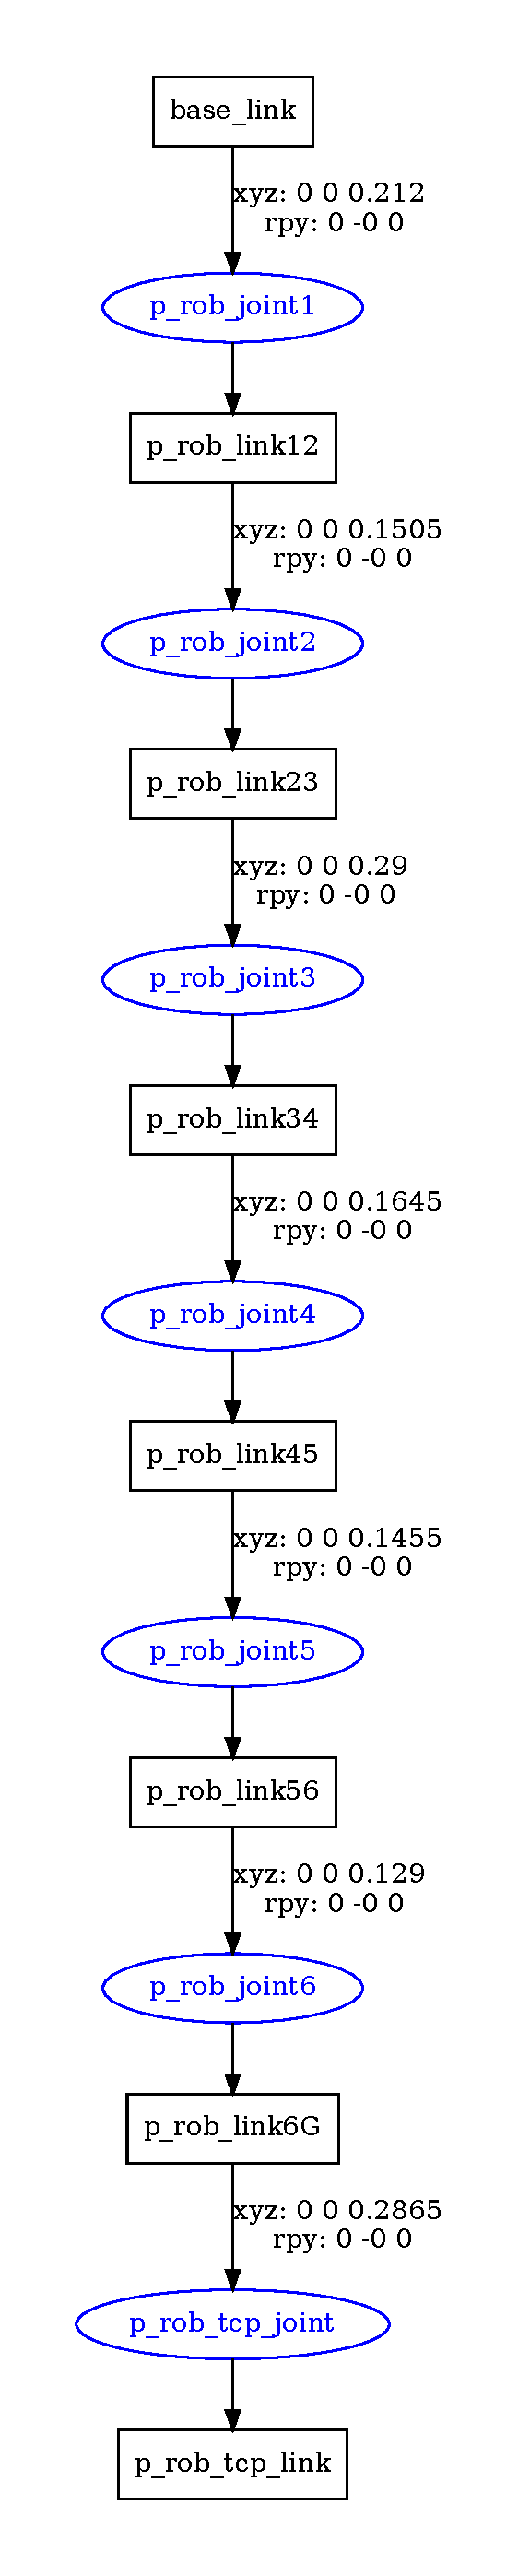
\includegraphics[width=0.3\linewidth]{./OtherFiles/p_rob.pdf}
	\caption{Catena cinematica descritta dal file urdf.}
	\label{fig:urdf_prob3}
\end{figure}
Nel file urdf, che è strutturato come un file xml, è possibile specificare i giunti e i link del robot tramite i seguenti elementi:
\begin{itemize}
	\item \tl link name="xxx"\tr...\tl /link\tr, descrive un link;
	\item \tl joint name="yyy" type="zzz"\tr...\tl /joint\tr, descrive un giunto; il robot utilizzato è costituito da sei giunti di rotazione, per cui il tipo dei giunti è definito come "revolute".
\end{itemize}
All'interno degli elementi è possibile poi specificare diverse caratteristiche tra le quali (elenco completo reperibile al link \url{http://wiki.ros.org/urdf/XML/joint}):
\begin{itemize}
	\item  \tl parent link="xxx"/\tr\ e \tl child link="yyy"/\tr\ indicano rispettivamente il link padre e il link figlio di un giunto;
	\item \tl axis xyz="0 1 0"/\tr\ indica l'asse di rotazione del giunto;
	\item  \tl origin xyz="0 0 0.29"/\tr\ indica la rototraslazione tra il link padre e il link figlio.
	\item \tl limit effort="1.09" lower="-2.94960643587" upper="2.9670597283903604" velocity="0.8290313946973065"/\tr \ descrive i limiti di velocità, angolo massimo e minimo e effort di un giunto;
\end{itemize}
Per descrivere il robot utilizzato, sono quindi stati definiti sei giunti di rotazione (tre con asse di rotazione lungo l'asse z e tre con asse di rotazione lungo l'asse y) e sette link dalla base del robot fino al centro di presa. Sono stati poi aggiunti un giunto di tipo \textit{fisso} e un link terminale per rappresentare correttamente il centro di presa.

\clearpage

\section{KDL paser}
A partire dalla descrizione del robot contenuta nel file urdf, è necessario costruire una struttura dati di tipo \texttt{KDL::Chain}, utilizzato dalla libreria Orocos KDL per i calcoli cinematici. Per fare ciò, si è utilizzato la libreria \textit{KDL parser}. Inizialmente, viene eseguito il parsing del file urdf tramite la funzione \texttt{urdf::parseURDFFile(path\_urdf)} che restituisce un oggetto di tipo urdf::ModelInterfaceSharedPtr che rappresenta il modello del file urdf. Se questa operazione viene effettuata correttamente, l'oggetto appena creato viene utilizzato per generare un oggetto di tipo \texttt{KDL::Tree} tramite la funzione \texttt{kdl\_parser::treeFromUrdfModel} che rappresenta la struttura del robot. Se l'oggetto viene creato correttamente, si utilizza il metodo \texttt{my\_tree.getChain("base\_link", "last\_link", m\_chain)} per definire un oggetto di tipo di tipo \texttt{KDL::Chain}, che rappresenta la catena cinematica del robot dal link "base\_link", il cui nome viene specificato come primo parametro della funzione, fino al link finale "last\_link", specificato come secondo parametro, che chiude la catena cinematica.

Successivamente, dall'oggetto \texttt{KDL::Chain} vengono estratti i limiti dei giunti (in termini di angoli minimi e massimi raggiungibili dai giunti). Essi vengono salvati in un array di tipo \texttt{KDL::JntArray} e saranno utilizzati nel calcolo della cinematica inversa.

\section{Sistemi di riferimento del robot}
Nelle figure \ref{fig:base_frame} e \ref{fig:tool_frame} sono riportati i sistemi di riferimento rispetto alla base del robot e del tool che sono stati considerati nel progetto. Inoltre le convenzioni scelte per indicare le rotazioni prevedono che gli angoli di roll (\textalpha), pitch (\textbeta) e yaw (\textgamma) siano definiti rispetto alla terna fissa (x,y,z) della base del robot, eseguendo le rotazioni nel seguente ordine: rotazione attorno all'asse x di angolo \textalpha, rotazione attorno all'asse y di angolo \textbeta\ e rotazione attorno all'asse z di angolo \textgamma.

\begin{figure}[tbh]
	\centering
	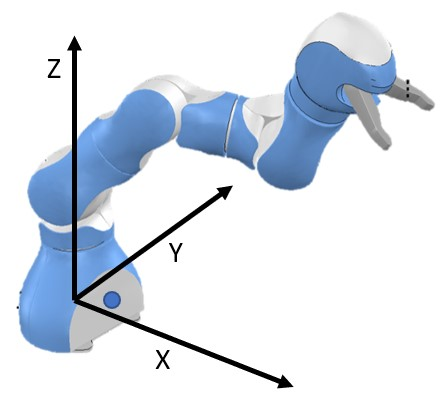
\includegraphics[width=0.5\linewidth]{./ImageFiles/prob_frame_base}
	\caption{Sistema di riferimento alla base del robot.}
	\label{fig:base_frame}
\end{figure}

\begin{figure}[tbh]
	\centering
	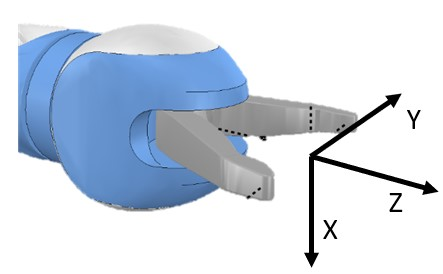
\includegraphics[width=0.5\linewidth]{./ImageFiles/prob_frame_tool.jpg}
	\caption{Sistema di riferimento del tool.}
	\label{fig:tool_frame}
\end{figure}

\clearpage

\section{Cinematica diretta}
La cinematica diretta permette di definire la posizione e l'orientamento dell'end-effector a partire dal valore dei giunti. La libreria Orocos KDL mette a disposizione il metodo \\ \texttt{int KDL::ChainFkSolverPos\_recursive::JntToCart(const JntArray\& q\_in, Frame\& p\_out)} \\ che riceve in ingresso un vettore di tipo \texttt{KDL::JntArray} che contiene la configurazione dei giunti e restituisce la posizione dell'end-effector rispetto al sistema del riferimento della base tramite l'oggetto \texttt{KDL::Frame}, che rappresenta una rototraslazione nello spazio 3D. Questo metodo appartiene alla classe \texttt{KDL::ChainFkSolverPos\_recursive} che implementa un algoritmo ricorsivo per il calcolo della cinematica diretta e il costruttore richiede come parametro un oggetto \texttt{KDL::Chain}. Il valore intero restituito indica l'esito del calcolo della cinematica diretta (zero se il calcolo è stato effettuato con successo).

\section{Cinematica inversa}
La cinematica inversa permette di ottenere la configurazione dei giunti a partire dalla posizione dell'end-effector espressa nel sistema di riferimento della base. La libreria Orocos 
KDL mette a disposizione diversi risolutori che implementano differenti algoritmi per il calcolo della cinematica inversa tramite metodi iterativi. In questo progetto è stato utilizzato il risolutore \texttt{KDL::ChainIkSolverPos\_NR\_JL} che implementa un metodo generale per la risoluzione della cinematica inversa utilizzando il metodo di Newton-Raphson tenendo in considerazione i limiti dei giunti. Il costruttore del risolutore ha la seguente segnatura: \texttt{KDL::ChainIkSolverPos\_NR\_JL::ChainIkSolverPos\_NR\_JL(const Chain \&\ chain, const JntArray \&\ q\_min, const JntArray \&\ q\_max, ChainFkSolverPos \&\ fksolver, \\ ChainIkSolverVel \&\ iksolver, unsigned int	maxiter = 100, double eps = 1e-6)}, dove chain è un oggetto di tipo \texttt{KDL::Chain} che corrisponde alla descrizione della catena cinematica del robot, q\_min e q\_max corrispondono contengono i limiti dei giunti, fksolver rappresenta un riferimento a un risolutore della cinematica diretta, iksolver un riferimento a un risolutore della cinematica inversa (nel progetto è stato utilizzato un risolutore di tipo KDL::ChainIkSolverVel\_pinv), maxiter rappresenta il numero massimo di iterazioni e eps rappresenta il massimo errore espresso in metri della posizione raggiunta dall'end-effector con i valori degli angoli ottenuti. Nel progetto sono stati scelti un numero di iterazione massimo pari a 1000 e una precisione di \SI{1}{\milli\meter}. 

La classe \texttt{KDL::ChainIkSolverPos\_NR\_JL} fornisce il metodo \\
\texttt{int KDL::ChainIkSolverPos\_NR\_JL::CartToJnt(const JntArray \&\ q\_init, const Frame \&\ p\_in, JntArray \&\	q\_out)} \\ che data la posizione dell'end-effector tramite il parametro p\_in, restituisce i valori dei giunti calcolati nella variabile q\_out. Il parametro q\_init rappresenta la configurazione iniziale dei giunti dalla quale il metodo iterativo inizia la ricerca della soluzione della cinematica inversa. Il valore intero restituito indica l'esito dell'operazione (zero se il calcolo è andato a buon fine).

\section{Traiettoria lineare}
\todo{spiegare la funzione path line e i metodi associati}

\chapter{Implementazione in STAR} \todo{nome solo per far capire la sezione (es diagramma componeti)}
\section{Plugin: PluginArmPRob3Kinematics}
\todo{descrivere funzioni plugin richiamando le funzioni della libreria}
\section{Componente: ArmDriver e ToolInput}
\todo{funzionamento dei due componenti/messaggi scambiati}
